\documentclass[paper=a4,11pt,titlepage,twoside=true,headings=normal,numbers=noenddot,captions=tableabove,listof=totoc,index=totoc,bibliography=totoc]{scrreprt}
%\usepackage{amsmath} % abgesetzte Formeln zentriert in der Zeile
%\usepackage[fleqn,intlimits]{amsmath} % [fleqn] abgesetzte Formeln mit festem Abstand zum linken Rand
\usepackage[reqno,intlimits]{amsmath} % [reqno] um die gleichungsnummerierung rechts zu haben
% intlimits: Grenzen für Integrale unterhalb und oberhalb des Zeichens
\usepackage{amssymb}
\usepackage{array}
\usepackage[ngerman]{babel}
\usepackage[ngerman]{varioref}
\usepackage[T1]{fontenc} 
\usepackage[utf8]{inputenc}
%---------------------------
\usepackage{booktabs}
\usepackage{calc}
\usepackage{cancel}
\usepackage[labelfont={footnotesize,sf,bf},textfont={footnotesize,sf}]{caption} %Format (Textgröße, Textform) für Bildtext 
%normalsize
%scriptsize
% sc --> smallcaps
% bf --> bold face
% sf --> sans serif
%\usepackage{cleveref} % löscht labels!!!!!!!!!!
%\usepackage{cite} %inkompatibel mit biblatex
\usepackage[table]{xcolor}
%\usepackage{colortbl}
\usepackage[right]{eurosym}
%\usepackage{caption2} %nicht zusammen mit sidecap
%\usepackage{exscale}
\usepackage{ellipsis}
\usepackage{graphicx}
\usepackage{float}
%\usepackage{floatflt}
%----------------------------------------
\usepackage{gensymb} %-----------
%\usepackage{helvet}
\usepackage{csquotes}
\usepackage{listings}
\usepackage{longtable}
\usepackage{lastpage}  %----------
\usepackage{lscape}
\usepackage{lmodern}  %-- Silbentrennung
%\usepackage{mathpazo} % andere mathematische Symbol
\usepackage{makeidx}
%\usepackage{minitoc}
\usepackage{multirow}
\usepackage{multicol}
%\usepackage[intoc]{nomencl}   % zwei Spalten beim Formelzeichenverzeichnis
\usepackage[german,intoc]{nomentbl} %vier Spalten bei Formelzeichenverzeichnis
\usepackage{nicefrac} %----
%\usepackage{picins} %----------
\usepackage{paralist} %--------
\usepackage{parallel}  %----------
\usepackage{pdfpages} %-------
% Define user colors using the RGB model
%\usepackage{colortbl}
%\definecolor{dunkelgrau}{rgb}{0.8,0.8,0.8}
%\definecolor{hellgrau}{rgb}{0.95,0.95,0.95}
%\usepackage{pgfplots}
\usepackage[figuresright]{rotating} 
\usepackage{scrlayer-scrpage}
%\usepackage[innercaption]{sidecap} %Beschriftung neben Bild, Tabelle, Mittelbach S333 %----------
%\usepackage{sistyle}
%\usepackage[locale=DE]{siunitx} %nicht zusammen mit sistyle %---------
\usepackage[locale=DE,per-mode=symbol,parse-numbers=false]{siunitx} %nicht zusammen mit sistyle %---------
\usepackage[font={scriptsize,sl},captionskip=3pt]{subfig} % für die Unterbilder %---------
\usepackage{shortvrb}
\usepackage{tablefootnote}
\usepackage{tabularx}
\usepackage{tabulary}
\usepackage{textcomp}
\usepackage{tocbasic}
%\usepackage{tikz}
\usepackage{times} 
\usepackage{units} %----------
\usepackage{url}
\usepackage{wrapfig} %----------
\usepackage{xr-hyper}
\usepackage{arydshln} %für \hdashline[5pt/2pt] % muss am Ende stehen, sonst gibt es Probleme mit xcolor
\usepackage{hyperref} % muss am Schluss stehen
\hypersetup{linkcolor={0 1 1}, linkbordercolor={1 1 1}, citebordercolor={1 1 1}} % setzt Linkboxen auf Farbe "`weiß"'
%\usepackage{bm}
%\usepackage[toc,symbols]{glossaries} %---------- muss nach hyperref stehen
\usepackage[nonumberlist, acronym, toc, section]{glossaries} % muss nach hypersetup stehen
%----------------
%\usepackage{romannum} % Seitenzahlen in römischen Ziffern
%\usepackage{adjustbox}
\usepackage{scrhack}
% \usepackage[square]{natbib}
\usepackage[style=numeric, citestyle=numeric, backend=biber]{biblatex}
%-------------------------
 %\renewcommand{\captionlabelfont}{\sffamily} %für "Abbildung" und "Tabelle"
 %\renewcommand{\captionfont}{\sffamily\small} %für den Text der Bildunterschriften
%  \renewcommand{\captionlabelfont}{\sffamily} 
%  \renewcommand{\captionfont}{\sffamily} %\renewcommand{\normalfont}{\sffamily} %für die Überschriften
% Fettdruck der Bezeichnung Abbildung, Tabelle
%\renewcommand{\captionlabelfont}{\bfseries}
%---------------------------------------------
%------------------ Schrifttyp in der Kopf- und Fusszeilen
\setkomafont{pageheadfoot}{\footnotesize\sffamily}
%---------------------------------------------------
%Ändern der Abbildung- und Tabellenbezeichnung (Niedermair S.157)
%_____________________________________________
\addto\captionsngerman{\renewcommand\figurename{Abb.}}
\addto\captionsngerman{\renewcommand\tablename{Tab.}}
\renewcommand\listfigurename{Abbildungen}
%_______________________________
%Betrag eines Wertes
\newcommand{\abs}[1]{\lvert #1 \rvert} 
%---------------------------------------------
\newcommand{\absatz}[1]{\textbf{\textsc{#1}}} %siehe Mittelbach S. 876ff
%----------------------------
%\newcommand{\absatz}{\par \medskip}
%______________________________
%\newcommand{\anhang}[1]{Anhang \ref{#1}, Seite \pageref{#1}}
\newcommand{\anhang}[1]{Anhang \vref{#1}}
%________________________________
\newcommand{\aufgabe}{\stepcounter{plus} Aufgabe \arabic{plus}}
%______________________________________
%compactitem
\newcommand{\bci}{\begin{compactitem}}
\newcommand{\eci}{\end{compactitem}}
%______________________________________
%
\newcommand{\bi}{\begin{itemize}}
\newcommand{\ei}{\end{itemize}}
%______________________________________
%compactenumerate
\newcommand{\bce}{\begin{compactenum}}
\newcommand{\ece}{\end{compactenum}}
%_____________________________________
%begin equation
\newcommand{\be}{\begin{equation}}
\newcommand{\ee}{\end{equation}}
%_____________________________________
%begin equation ohne Formelnummer
\newcommand{\ben}{\begin{equation*}}
\newcommand{\een}{\end{equation*}}
%_____________________________________
%begin align ohne Formelnummer
\newcommand{\ban}{\begin{align*}}
\newcommand{\ean}{\end{align*}}
%_____________________________________
%begin align
\newcommand{\ba}{\begin{align} }
\newcommand{\ea}{\end{align}}
%_____________________________________
%minpage
\newcommand{\bmp}{\begin{minipage}[t]{.47\linewidth}}
\newcommand{\emp}{\end{minipage}}
%_____________________________
%  dB
\newcommand{\db}{dB}
%  dB(A)
\newcommand{\dba}{ dB(A) }
%  dB(A) für Satzende
\newcommand{\dbap}{ dB(A)}
%_________________________________
\newcommand{\bzw}{bzw.\,}
%_______________________________
\newcommand{\dif}{\mathrm{d}}
%________________________________
% neuer Zähler
\newcounter{plus}
\setcounter{plus}{0}
%______________________________
%Für das Formelverzeichnis _____________________ Formelverzeichis ____
% Befehl umbenennen in fz
\let\fz\nomenclature
% Deutsche Überschrift
\renewcommand{\nomname}{Formelzeichen}
% Punkte zw. Abkürzung und Erklärung
\setlength{\nomlabelwidth}{.20\hsize}
\renewcommand{\nomlabel}[1]{#1 \dotfill}
% Zeilenabstände verkleinern
\setlength{\nomitemsep}{-\parsep}
%_____________________________
\newcommand{\bild}[1]{Abb. \vref{#1}}
\newcommand{\sbild}[1]{siehe Abb. \vref{#1}}
\newcommand{\bilder}[2]{Abb. \vrefrange{#1}{#2}}
\newcommand{\bildseite}[1]{Abb. \vref{#1}} % erzeugt "`Abb. nn auf Seite nn
\newcommand{\tabelle}[1]{Tab. \vref{#1}}
\newcommand{\tabellenseite}[1]{Tab. \vref{#1}} % erzeugt "`Tab. nn auf Seite nn
% für \vref ist usepackage[german]{varioref} einzufügen
%_-------------------------------- Freiraum
\newcommand{\freiraum}[1]{\begin{figure}[H]\vspace{#1\textheight}\end{figure}}
%_____________________________
% Gleichung
\newcommand{\gl}[1]{Gl.\,(\ref{#1})}
\newcommand{\sgl}[1]{siehe Gl.\,(\ref{#1})}
\newcommand{\glbereich}[2]{Gl. \vrefrange[]{#1}{#2}}
%_____________________________
% Grad Celsius
\newcommand{\grad}{\,\degC}
\newcommand{\gradC}{\,\degree}
%______________________________________
% Großbuchstaben als Indizes kleiner schreiben; spezielle im Mathemodus
\newcommand{\klein}[1]{\scriptscriptstyle{#1}}% Fettdruck der Bezeichnung 
%______________________________
%% Kasten
\newcommand{\kasten}{\fbox{\rule{0.0pt}{10pt}{{ } } }}
%______________________________
%\newcommand{\kapitel}[1]{Kapitel \ref{#1}, Seite \pageref{#1}}
\newcommand{\kapitel}[1]{Kapitel \vref{#1}}
%_____________________________
%  LAeq für den äquivalenten Dauerschallpegel
\newcommand{\laeq}{ $L_{Aeq}$ }
%  LAeq für den äquivalenten Dauerschallpegel am Satzende
\newcommand{\laeqp}{ $L_{Aeq}$}
%_________________________________
%   Linie zeichnen
\newcommand{\linie}{\rule{0.5\textwidth}{0.1pt}}
%---------------------- LaTeX
\newcommand{\lt}{\LaTeX\,\,}
%----------------------------
\newcommand{\nl}{\newline}
%__________________________________
%  multicolumn für Tabellen
\newcommand{\mc}{\multicolumn}
%% \mc{1}{c}{Text}
%_________________________________
%    Parallel
\newcommand{\pl}[1]{\ParallelLText{#1}}
\newcommand{\pr}[1]{\ParallelRText{#1}}
\newcommand{\pp}{\ParallelPar}
%------------ rot unterstrichen
\newcommand{\rotunterstrichen}[1]{\textcolor{red}{\underline{\textcolor{black}{#1}}}}
%________________ Realteil
\newcommand{\real}[1]{\text{Re}\left\{#1\right\}}
%________________________________--
\newcommand{\seite}[1]{Seite \pageref{#1}}
\newcommand{\seiten}[2]{\vpagerefrange{#1}{#2}}
%----------------------------
%        TEXT Rot
\newcommand{\textrot}[1]{\textcolor{red}{#1}}
%______________________________
%Abkürzung für \multicolumn
\newcommand{\tab}[2]{\multicolumn{1}{#1}{#2}}
%_____________________________________
% doppelt unterstreichen
\newcommand{\unterstreichen}[1]{\underline{\underline{#1}}}
% einfach unterstreichen
\newcommand{\ul}[1]{\underline{#1}}
%______________________________
%kurze Verbatimausgabe
%\MakeShortVerb{\|} %mittelbach S.160 mit \usepackage{shortvrb}
%_______________________________________
% vspace
\newcommand{\vsf}{\vspace{5pt}}
%_________________________________
\newcommand{\zb}{z.B.\,}
\newcommand{\idr}{i.d.R.\,}
%_______________________________
% Zähler-einfach
\newcounter{req}
\newcommand{\zaehler}[1]{\refstepcounter{req}{#1} \thereq}
%% Beispielaufzählung \zaehler{Beispiel}\\
%_____________________________________
 \setlength{\voffset}{-2.532 cm}
 \setlength{\hoffset}{-1.57 cm}
% \setlength{\topmargin}{2.0 cm} \setlength{\topskip}{0.1 cm}
 \setlength{\topmargin}{1.5 cm}
 \setlength{\topskip}{0.1 cm}
 \setlength{\evensidemargin}{1.5 cm}
 \setlength{\oddsidemargin}{1.5 cm}
 \setlength{\textwidth}{16.5 cm}
 \setlength{\footskip}{40pt}
 \setlength{\textheight}{24.5cm}
% \setlength{\textheight}{23.5 cm}
 \setcounter{page}{1}
 \setlength{\parindent}{0cm}
 \setlength{\headsep}{20pt}
%----------------------------------------------------------------------
% Linien in der Kopf- und Fußzeile
%\renewcommand{\headrulewidth}{0.0pt}   %Linie in der Kopfzeile mit 0.0pt keine Linie
%%\renewcommand{\footrulewidth}{0.0pt}   %Linie in der Fußzeile mit 0.0 pt keine Linie
%\renewcommand{\headrulewidth}{0.2pt}   %Linie in der Kopfzeile mit 0.0pt keine Linie
%\renewcommand{\footrulewidth}{0.2pt}   %Linie in der Fußzeile mit 0.0 pt keine Linie
%------------------------------------------------------------------------
%\renewcommand{\normalfont}{\sffamily} %für die Überschriften
%\renewcommand{\chaptermark}[1]{\markboth{\chaptername\ \thechapter #1}{}}
%\renewcommand{\sectionmark}[1]{\markright{\thesection\ #1}}
% \rfoot{\leftmark\\\rightmark}

%Definitionen für Kopfzeile
% bei documentclass {report} hat der Eintrag für die [gerade Seite] keine Wirkung
%-------------------------------------------------------------
%%
%Einstellungen für Kopf- und Fusszeilen mit dem KOMA-Skript und \usepackage{scrpage2}
\pagestyle{scrheadings}
%\pagestyle{scrplain}
% le --> links, gerade Seite
% ce --> mittig, gerade Seite
% re --> rechts, gerade Seite
% lo --> links, ungerade Seite
% co --> mittig, ungerade Seite
% ro --> rechts, ungerade Seite
%---------------------------------------------
% Löschen aller Einträge
%\clearscrheadings
% \automark[section]{subsection}
% \pagemark --> Seitenzahl
% \automark --> Kapitelüberschriften
% \leftmark --> ??
% \rightmark --> ??
%::::::::::::::::::::::::::::::::::: Kopfzeile
% Kopfzeile gerade Seite
\automark[chapter]{chapter}
\lehead[]{\titelkopfzeilelinkseven}
\cehead[]{\titelkopfzeilemitteeven}
\rehead[]{\titelkopfzeilerechtseven}
% Kopfzeile ungerade Seite
\lohead[]{\titelkopfzeilelinksodd}
\cohead[]{\titelkopfzeilemitteodd}
\rohead[]{\titelkopfzeilerechtsodd}
% Linie in der Kopfzeile
%\setheadtopline{0.2pt} % obere Linie in der Kopfzeile; nur bei scrartcl
\setheadsepline{0.4pt} % untere Linie in der Kopfzeile; nur bei scrartcl
% Linie in der Fusszeile
%::::::::::::::::::::::::::::::::::: Fußzeile
% Fusszeile gerade Seite[plain-style]{scrheadings-style}
\lefoot[]{\titelfusszeilelinkseven} 
\cefoot[]{\titelfusszeilemitteeven}
\refoot[]{\titelfusszeilerechtseven}
% Fusszeile ungerade Seite
\lofoot[]{\titelfusszeilelinksodd}
\cofoot[]{\titelfusszeilemitteodd}
\rofoot[]{\titelfusszeilerechtsodd}
%\rofoot[\thepage ]{\thepage}
%\setfoottopline{0.2pt} % obere Linie in der Kopfzeile; nur bei scrartcl
\setfootsepline{0.4pt} % untere Linie in der Kopfzeile; nur bei scrartcl

% le --> links, gerade Seite
% ce --> mittig, gerade Seite
% re --> rechts, gerade Seite
% lo --> links, ungerade Seite
% co --> mittig, ungerade Seite
% ro --> rechts, ungerade Seite
% even --> gerade Seite
% odd --> ungerade Seite
%----------------------------------------- Kopfzeilentext
 \newcommand{\titelkopfzeilemitteeven}{}
 \newcommand{\titelkopfzeilemitteodd}{}
 \newcommand{\titelkopfzeilelinkseven}{Hochschule RheinMain}
 \newcommand{\titelkopfzeilelinksodd}{}
 \newcommand{\titelkopfzeilerechtseven}{}
 \newcommand{\titelkopfzeilerechtsodd}{Hochschule RheinMain}
 %----------------------------------------- Fußzeilentext
 \newcommand{\titelfusszeilemitteeven}{}
 \newcommand{\titelfusszeilemitteodd}{}
 \newcommand{\titelfusszeilerechtseven}{Studienbereich Angewandte Physik \& Medizintechnik}
 \newcommand{\titelfusszeilerechtsodd}{\thepage \hspace{0.5mm} von \pageref{LastPage}}
 \newcommand{\titelfusszeilelinkseven}{\thepage \hspace{0.5mm} von \pageref{LastPage}}
 \newcommand{\titelfusszeilelinksodd}{Studienbereich Angewandte Physik \& Medizintechnik}
\newcommand{\titelLV}{Physikalisches Praktikum 2}
%---------------------------- VARIABLEN festlegen ------------------
%----------- Pro Versuch zu ändernde Angaben -----------------------
\newcommand{\versuch}{1} % Versuchsnummer einfügen
\newcommand{\untertitelb}{Magnetfeldmessung} % Titel des Versuchs einfügen
\newcommand{\datumLV}{19.10.2020} % Datum einfügen
\newcommand{\deadline}{2.11.2020} % Datum einfügen
%----------- TITEL
\newcommand{\untertitela}{Versuch P2-3}
% -------- Student 1
\newcommand{\nameA}{Herr Cihan Ünlü}
% --------- Student 2
\newcommand{\nameB}{Herr Dennis Hunter}
% --------- Student 3, falls vorhanden
\newcommand{\nameC}{Herr Student drei}
%::::::::::::::::::::::::::::::::::
%\input{chapters/glossar}
\addbibresource{quellen.bib}
\begin{document}
%-----------------------------------------------------------------
\begin{titlepage} 
	\newcommand{\HRule}{\rule{\linewidth}{0.5mm}} 	
	\centering
	\textsc{\Large Hochschule RheinMain \\
		
\includegraphics[width=0.15\textwidth]{logo-hsrm}\\[1cm]}
%	\textsc{\Large Hochschule RheinMain}\\[1cm]
	\textsc{\LARGE \titelLV}\\[0.5cm]
		\HRule\\[0.4cm]
	{\huge\bfseries \untertitela}\\[0.4cm] % Title des Dokuments
	{\huge\bfseries \untertitelb}\\[0.4cm] % Title des Dokuments
		\HRule\\[1.5cm]
%-------------------
%\begin{flushleft}
	\begin{minipage}{0.4\textwidth}
%	\begin{flushleft}
%\centering
		\large
		\textit{\underline{Autoren}}\\[0.5cm]
		\textsc{\nameA}\\[0.5cm]
		\textsc{\nameB}\\[0.5cm]
		%\textsc{\nameC}\\[0.5cm] 
%	\end{flushleft}
\end{minipage}
%------------------------------------
\vfill\vfill\vfill 
\textsc{\Large Fachbereich Ingenieurwissenschaften}\\[0.5cm]
\textsc{\large Studienbereich Angewandte Physik \& Medizintechnik}\\[0.5cm] 
\vfill	
Datum des Versuchs:\hspace{0.4cm} {\large\datumLV}\\
Abgabedatum:\hspace{0.4cm} {\large\deadline} 
\end{titlepage}

%-----------------------------------------------------
\tableofcontents
\newpage
%--------------------
\chapter{Einleitung}
%Ziel des Versuchs.
Ziel des Versuches ist es, die magnetische Feldstärkern im Zentrum der magnetischen Achsen verschiedener Zylinderspulen
in Abhängigkeit ihrer Geometrien und Windungszahlen zu untersuchen.

\section{Grundlagen}
%Phys. und Messtechn. Grundlagen
Wird ein Permanentmagnet in ein äußeres magnetisches Feld eingebracht wirkt auf ihn eine Kraft, die seine magnetische
Achse entlang der äußeren Feldlinien ausrichtet. Im durchgeführten Versuch wird eine Magnetometer verwendet dessen
Funtionsprinzip sich diesen Effekt zunutze macht.
\par
\hspace{1cm}Ein Stabmagnet wird so innerhalb einer Zylinderspule angebracht, dass die magnetischen Achsen orthogonal und ihre
jeweiligen Mittelpunkte möglichst nah beieinander sind. Während das äußere Feld der Spulen ein Drehmoment bewirkt,
verursacht ein als Torsionsfeder dienender Draht ein Drehmoment in entgegen gesetzter Richtung (vgl. \gl{eq:7}).
\par
\hspace{1cm}Die resultierende Auslenkung wird durch einen an der Rotationsachse des Stabmagneten angebrachten Spiegel sichtbar
gemacht - ein stationärer Laserstrahl wird auf eine mit der Rotationsachse kozentrischen Skala analog zur derzeitigen
Auslenkung gebrochen.

\section{Gleichungen und Herleitungen}
%Herleitung der gegebenen Gl. aus den Grundgleichungen.
Die magn. Feldstärke innerhalb einer Spule kann durch \gl{eq:1} beschrieben werden.
\begin{equation}
    H(x) = \frac{I \cdot n}{2L} \left[ \cos{\beta} + \cos{\gamma} \right] = \frac{I \cdot n}{2L} \cdot \left[ \frac{ \frac{L}{2} - x}{ \sqrt{ \left(\frac{L}{2} - x \right)^2 + R^2 }} + \frac{ \frac{L}{2} + x}{ \sqrt{ \left(\frac{L}{2} + x \right)^2 + R^2 }} \right]
    \label{eq:1}
\end{equation}

\begin{figure}[h]
    \centering
    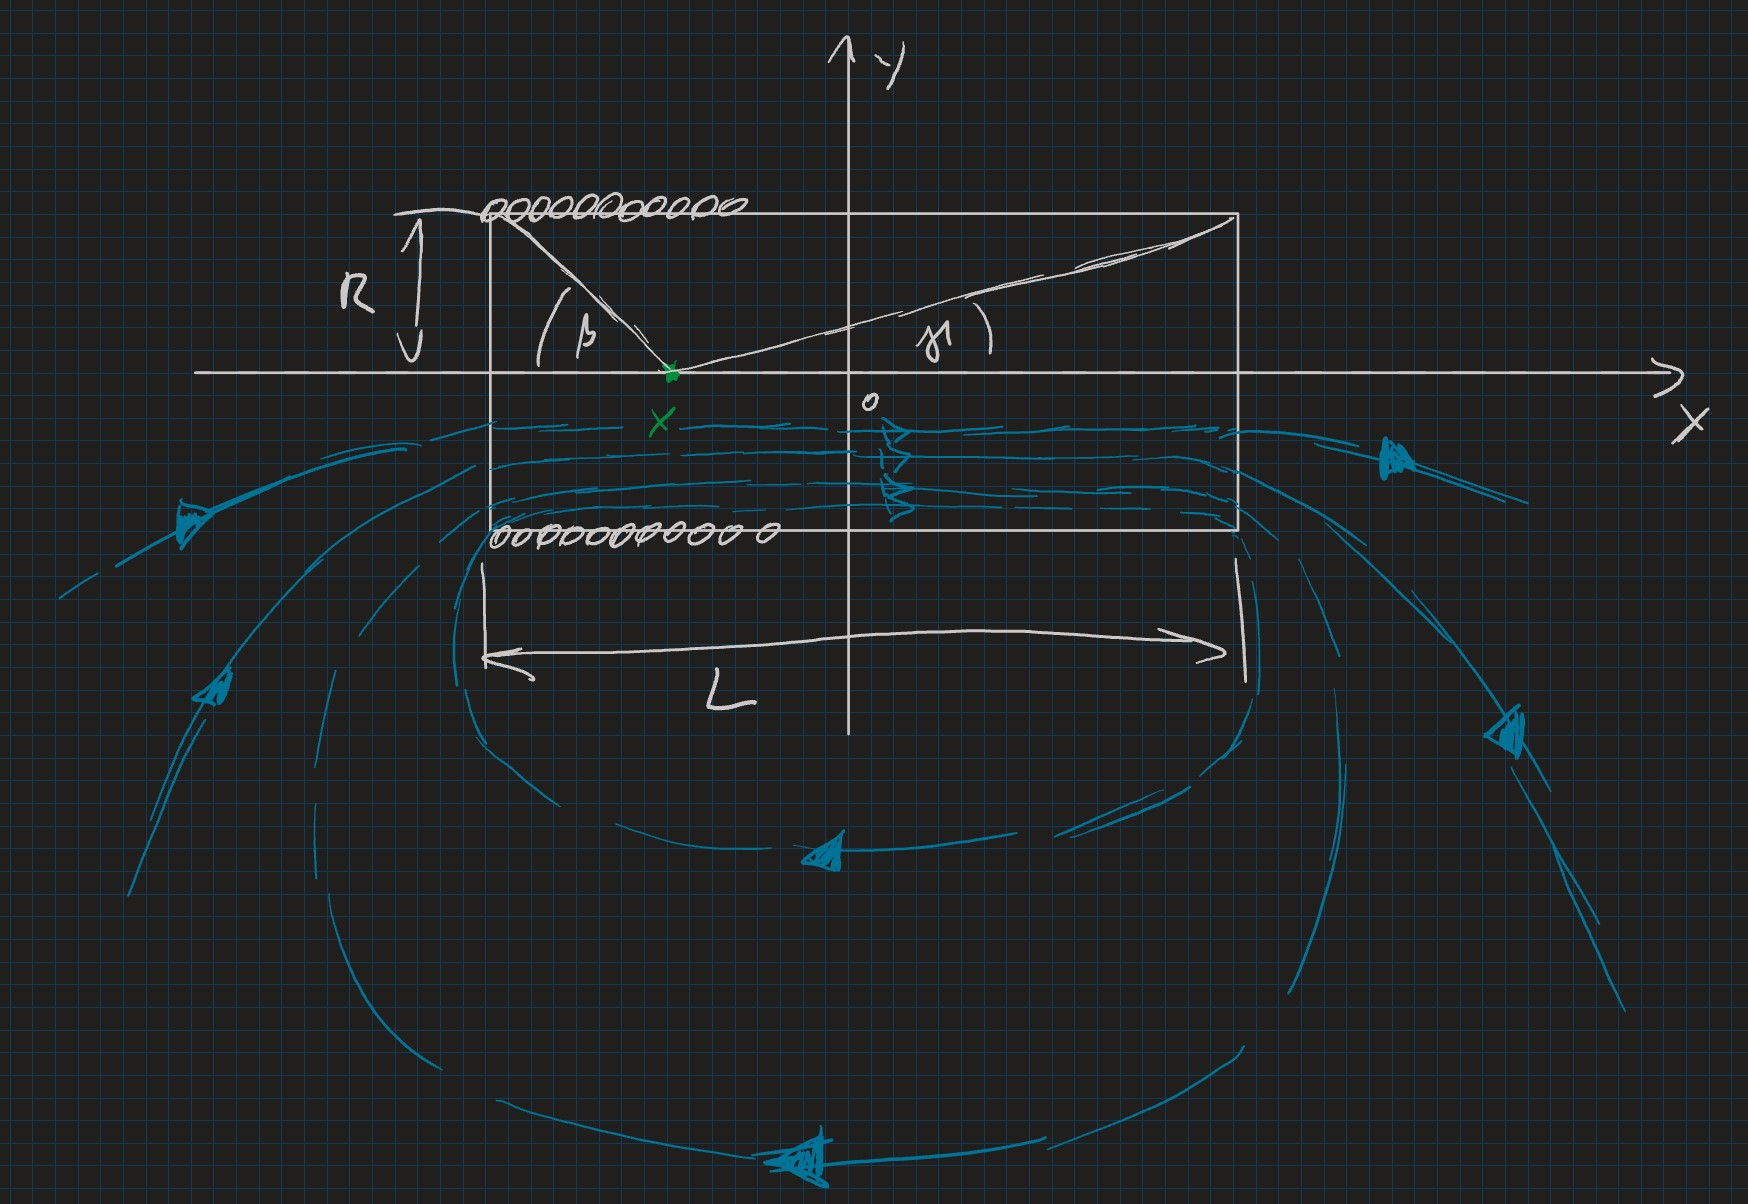
\includegraphics[width=.5\textwidth]{assets/feldInSpule.jpg}
    \label{fig:feldInSpule}
    \caption[Feld innerhalb einer Zylinderspule]{Schematische Darstellung des magnetischen Feldes innerhalb einer Zylinderspule.}
\end{figure}

An der Stelle $ x=0 $ vereinfacht sich \gl{eq:1} zu
\begin{equation}
    H(0) = \frac{I \cdot n}{2} \cdot \left[ \left( \frac{L}{2} \right)^2 + R^2 \right]^{-\frac{1}{2}}
    \label{eq:2}
\end{equation}

Im Falle einer langen Spule ist der Radius im Verhältnis zur Länge als vernachlässigbar klein anzunehmen. Wenn $ R\ll L$
gilt also in guter Näherung

\begin{equation}
    H_{l}(0)    = \frac{I \cdot n}{2} \cdot \left[ \left( \frac{L}{2} \right)^2 + \cancel{R^2} \right]^{-\frac{1}{2}}
                = \frac{I \cdot n}{2} \cdot \left( L \cdot \frac{1}{2} \right)^{-1}
                = \frac{I \cdot n}{L}
    \label{eq:3}
\end{equation}

Kehren sich die Verhältnisse um wird von einer kurzen Spule gesprochen und mit $ R \gg L$ gilt analog
\begin{equation}
    H_{k}(0)    = \frac{I \cdot n}{2} \cdot \left[ \left( \cancel{\frac{L}{2}} \right)^2 + {R^2} \right]^{-\frac{1}{2}}
                = \frac{I \cdot n}{2R}
    \label{eq:4}
\end{equation}
\par\bigskip

Für die Kraft zwischen zwei magn. Polen gilt (analog zur Elektrostatik) \cite{Unbekannt}\cite{Halliday.2005}

\begin{equation}
    F_{mag} = \frac{1}{4\pi \mu_0} \cdot \frac{\phi_1 \cdot \phi_2}{r^2}
    \label{eq:5}
\end{equation}

Ist hierbei $\phi_1$ der Stabmagnet und das Feld innerhalb der Spule mit \(\phi_2 = \vec{B} \bullet \vec{A}\) als vollkommen
homogen angenommen ergibt sich \gl{eq:5} zu

\begin{equation}
    F_{mag} = \phi_1 \cdot H \quad \text{mit} \quad
    H = \frac{1}{4\pi \mu_0} \cdot \frac{\phi_2}{r^2}
    \label{eq:6}
\end{equation}

\begin{figure}[h]
    \centering
    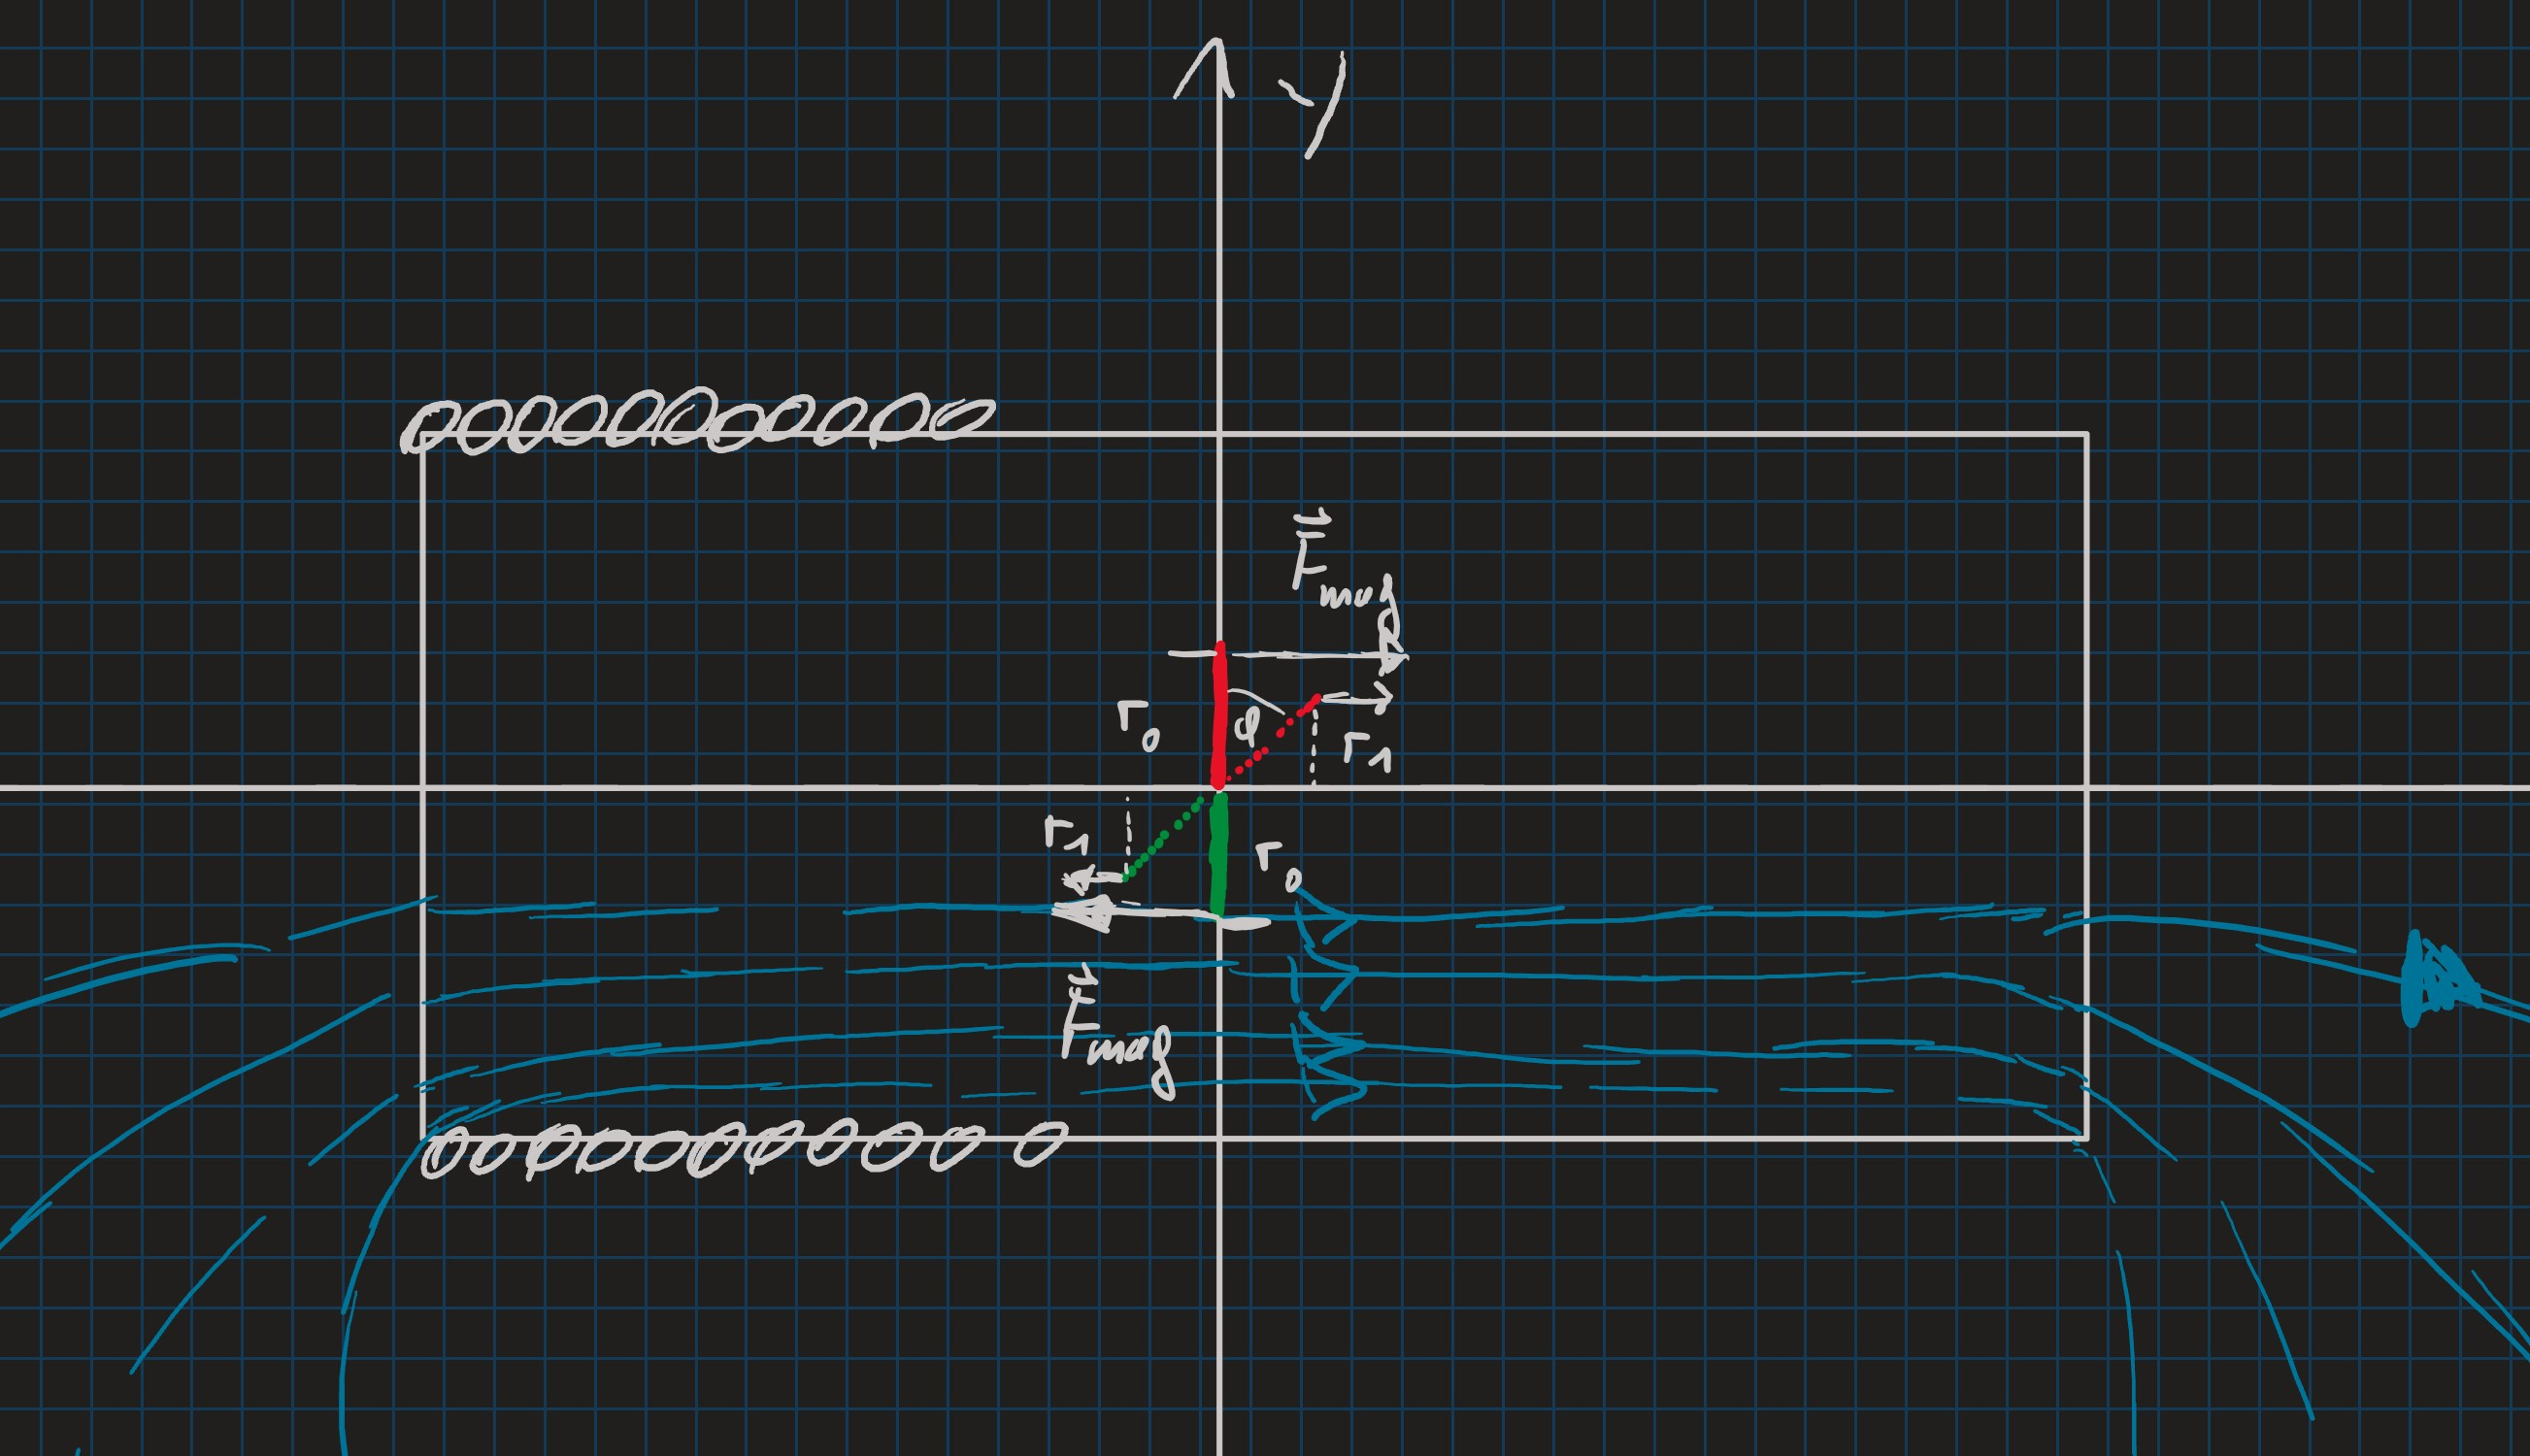
\includegraphics[width=.8\textwidth]{assets/drehmoment.jpg}
    \caption[Kräfte auf einen Stabmagnet im Magnetfeld]{Schematische Darstellung der wirkenden Kräfte auf den Stabmagnet innerhalb der Spule.}
    \label{fig:drehmoment}
\end{figure}
Hiermit und mit $\vec{M} = \vec{r} \times \vec{F}$ lässt sich das auf den Torsionsdraht wirkende Drehmoment ausdrücken durch (vgl. \bild{fig:drehmoment})
\begin{equation}
    M_{mag} = 2 \cdot F_{mag} \cdot r \cdot \cos{\varphi}
    = F_{mag} \cdot s \cdot \cos{\varphi}
    = \phi_1 \cdot H \cdot s \cdot \cos{\varphi}
    \label{eq:7}
\end{equation}
% \par\bigskip

Der Torsionsdraht selbst erzeugt ein umso größeres Rückstellmoment \(M_{Rück} = d \cdot \varphi\), je größer seine Verwindung - also \(\varphi\) - ist.
Ein Kräftgleichgewicht herrscht bei dem Auslenkungswinkel $\varphi$, bei dem die beiden Drehmomente gleich groß sind.
Es folgt durch Gleichsetzen beider Drehmomente und umstellen nach $\varphi$ 
\begin{equation*}
    \phi_1 \cdot H \cdot s \cdot \cos{\varphi} = d \cdot \varphi \quad \Leftrightarrow \quad \varphi = \frac{\phi_1 \cdot H \cdot s \cdot \cos{\varphi}}{d}
\end{equation*}

Unter der Annahme, dass die zu erwartenden Auslenkwinkel ausreichend klein sind verschwindet $\cos{\varphi}$ und es bleibt
\begin{equation}
    \varphi = \frac{\phi_1 \cdot H \cdot s}{d}
    \label{eq:8}
\end{equation}
\chapter{Versuchsaufbau}
\begin{figure}[ht]
    \centering
    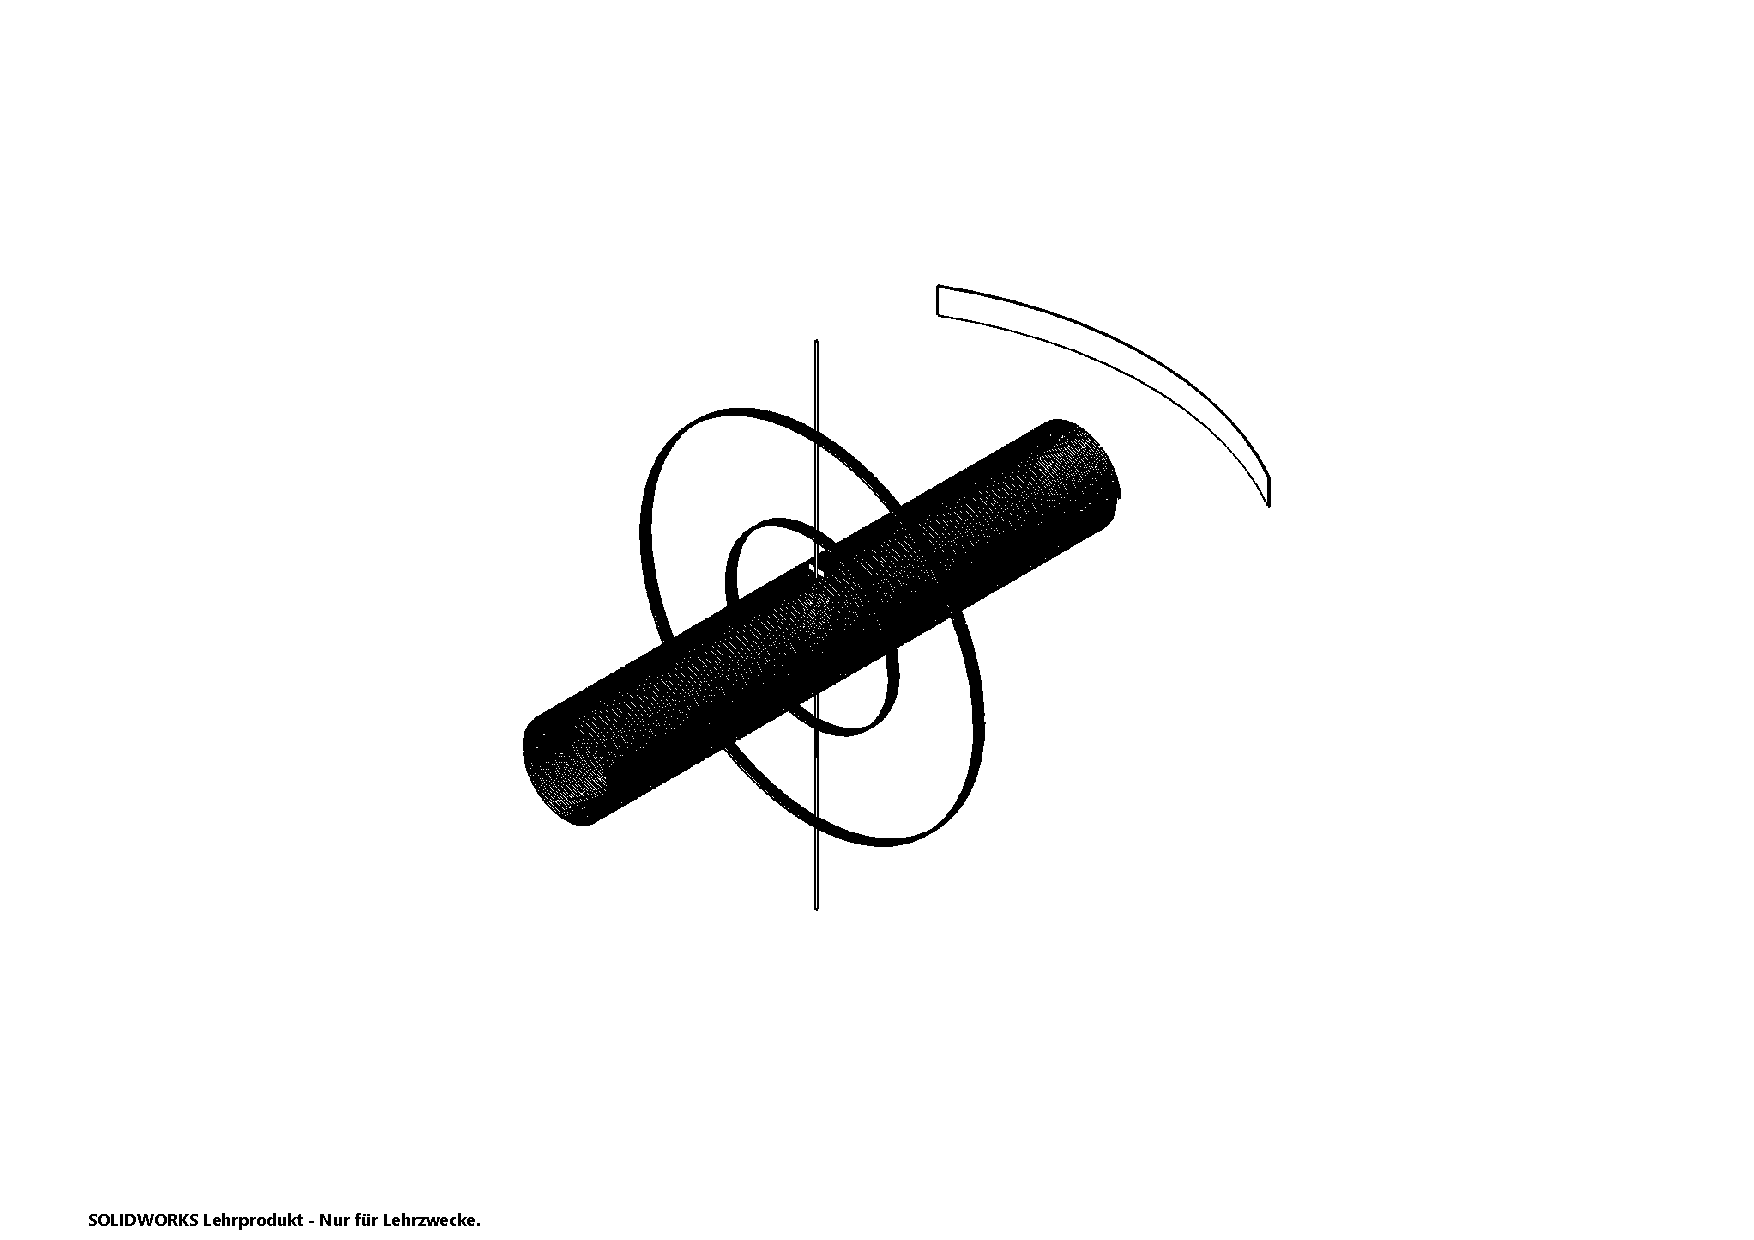
\includegraphics[width=.71\textwidth]{assets/Aufbau.jpg}
    \label{fig:aufbau}
    \caption[Versuchsaufbau]{Schematische Darstellung des Versuchsaufbaus und Kennzeichnung der wichtigsten funktionellen Komponenten.}
\end{figure}

\begin{figure}[ht]
    \centering
    \includegraphics[width=\textwidth]{assets/Aufbau_isometrisch.jpg}
    \label{fig:aufbau_iso}
    \caption[Versuchsaufbau - isometrisch]{Versuchsaufbau in isometrischer Ansicht.}
\end{figure}
\input{chapters/4_durchführung}
\chapter{Auswertung}
\section{Bestimmung des Kalibrierfaktors}
Da bedingt durch die Spulengeometrie das Feld innerhalb der langen Spule quantitativerseits Stärker und qualitativerseits
homogener als jenes der kurzen Spulen zu erwarten ist, dienen die Messungen an der langen Spule zur Ermittlung eines
Kalibrierfaktors $k$.\par
Mit Hilfe des Kalibrierfaktors lässt sich aus den gemessenen Ausschlägen die Feldstärke der kurzen Spulen gemäß 
\begin{equation}
    k=\frac{\Delta A}{\Delta H} \quad \Leftrightarrow \quad H=\frac{A}{k}
    \label{eq:k}
\end{equation}
ermitteln.

\begin{figure}[H]
    \centering
    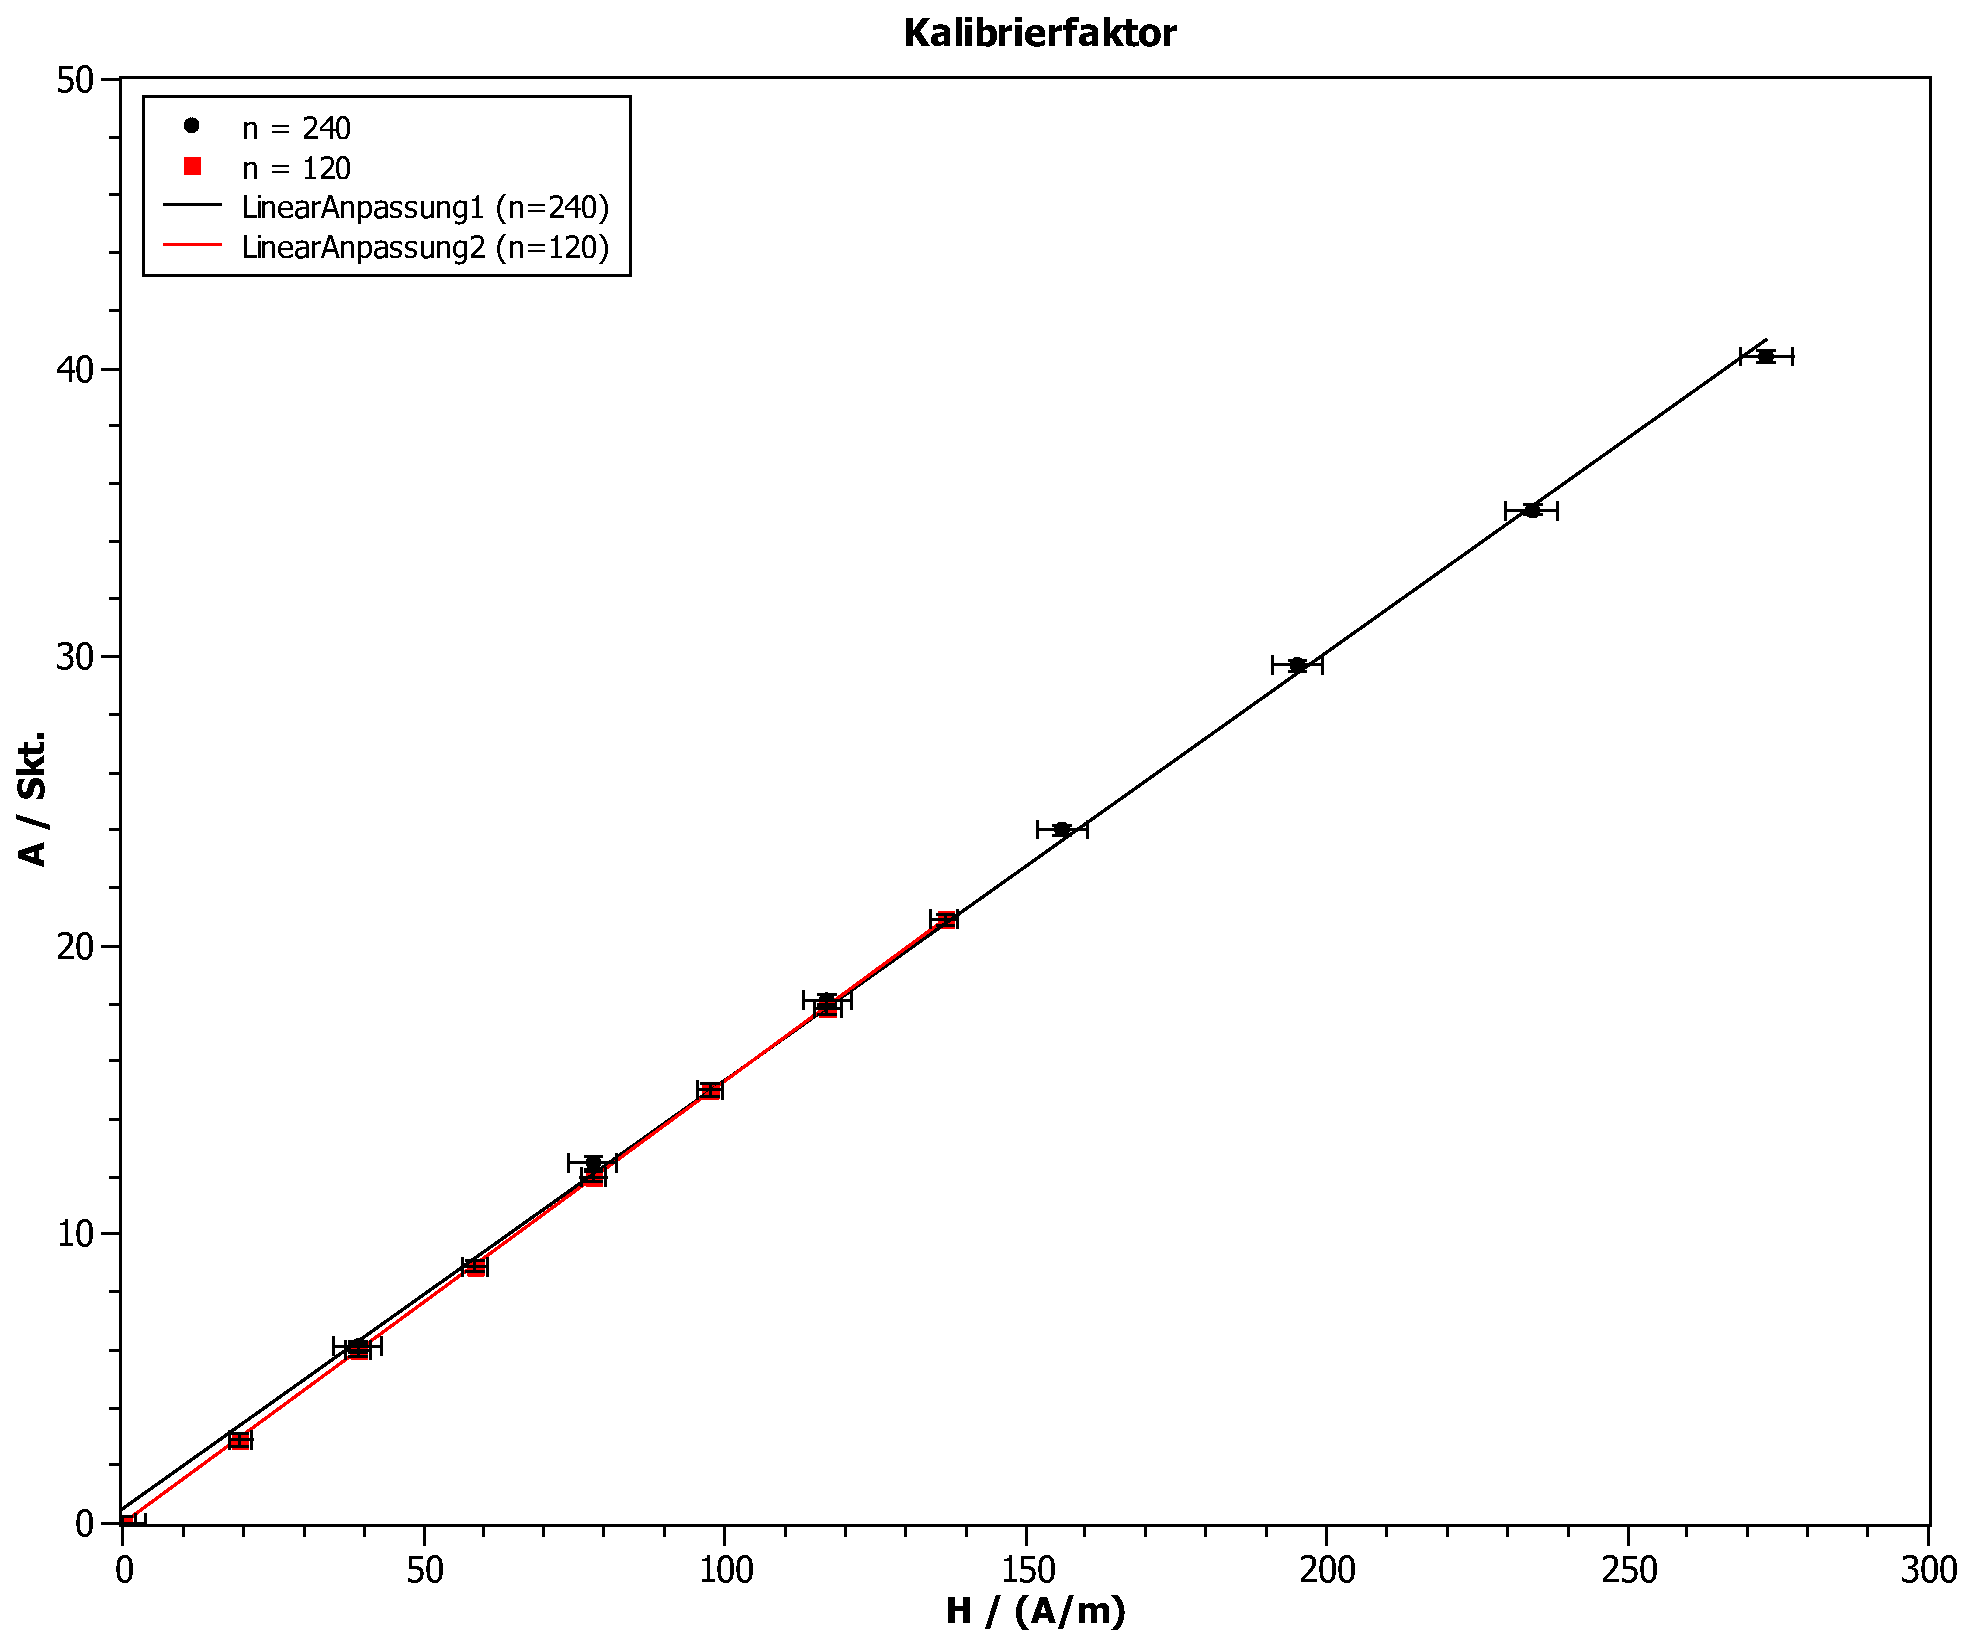
\includegraphics[width=.7\textwidth]{Kalibrierfaktor.pdf}
    \caption[Ermittlung des Kalibrierfaktors]{Ermittlung des Kalibrierfaktors als Steigung von $H_{l}(I)$ mittels \textsc{SciDavis} zur weiteren Auswertung der kurzen Spulen.}
    \label{fig:kalib}
\end{figure}

Wird der Spulenstrom $ I $ der langen Spule nach \gl{eq:3} in die magnetische Feldstärke $ H $ umgerechnet und der Skalenwert
$ A $ als Funktion von $ H $ in ein Diagramm (vgl. \bild{fig:kalib}) aufgetragen, so ergibt sich als Steigung der linearen
Anpassung der Kalibrierfaktor $ k $ mit der Abweichung $ \Delta k $

\begin{equation} 
    k = (0,151 \pm 0,002)\SI{}{\frac{Skt\cdot m}{A}}
\end{equation}

\section{Bestimmung des Proportionalitätsfaktors}

\begin{figure}[H]
    \hspace{-5mm}
    \centering
    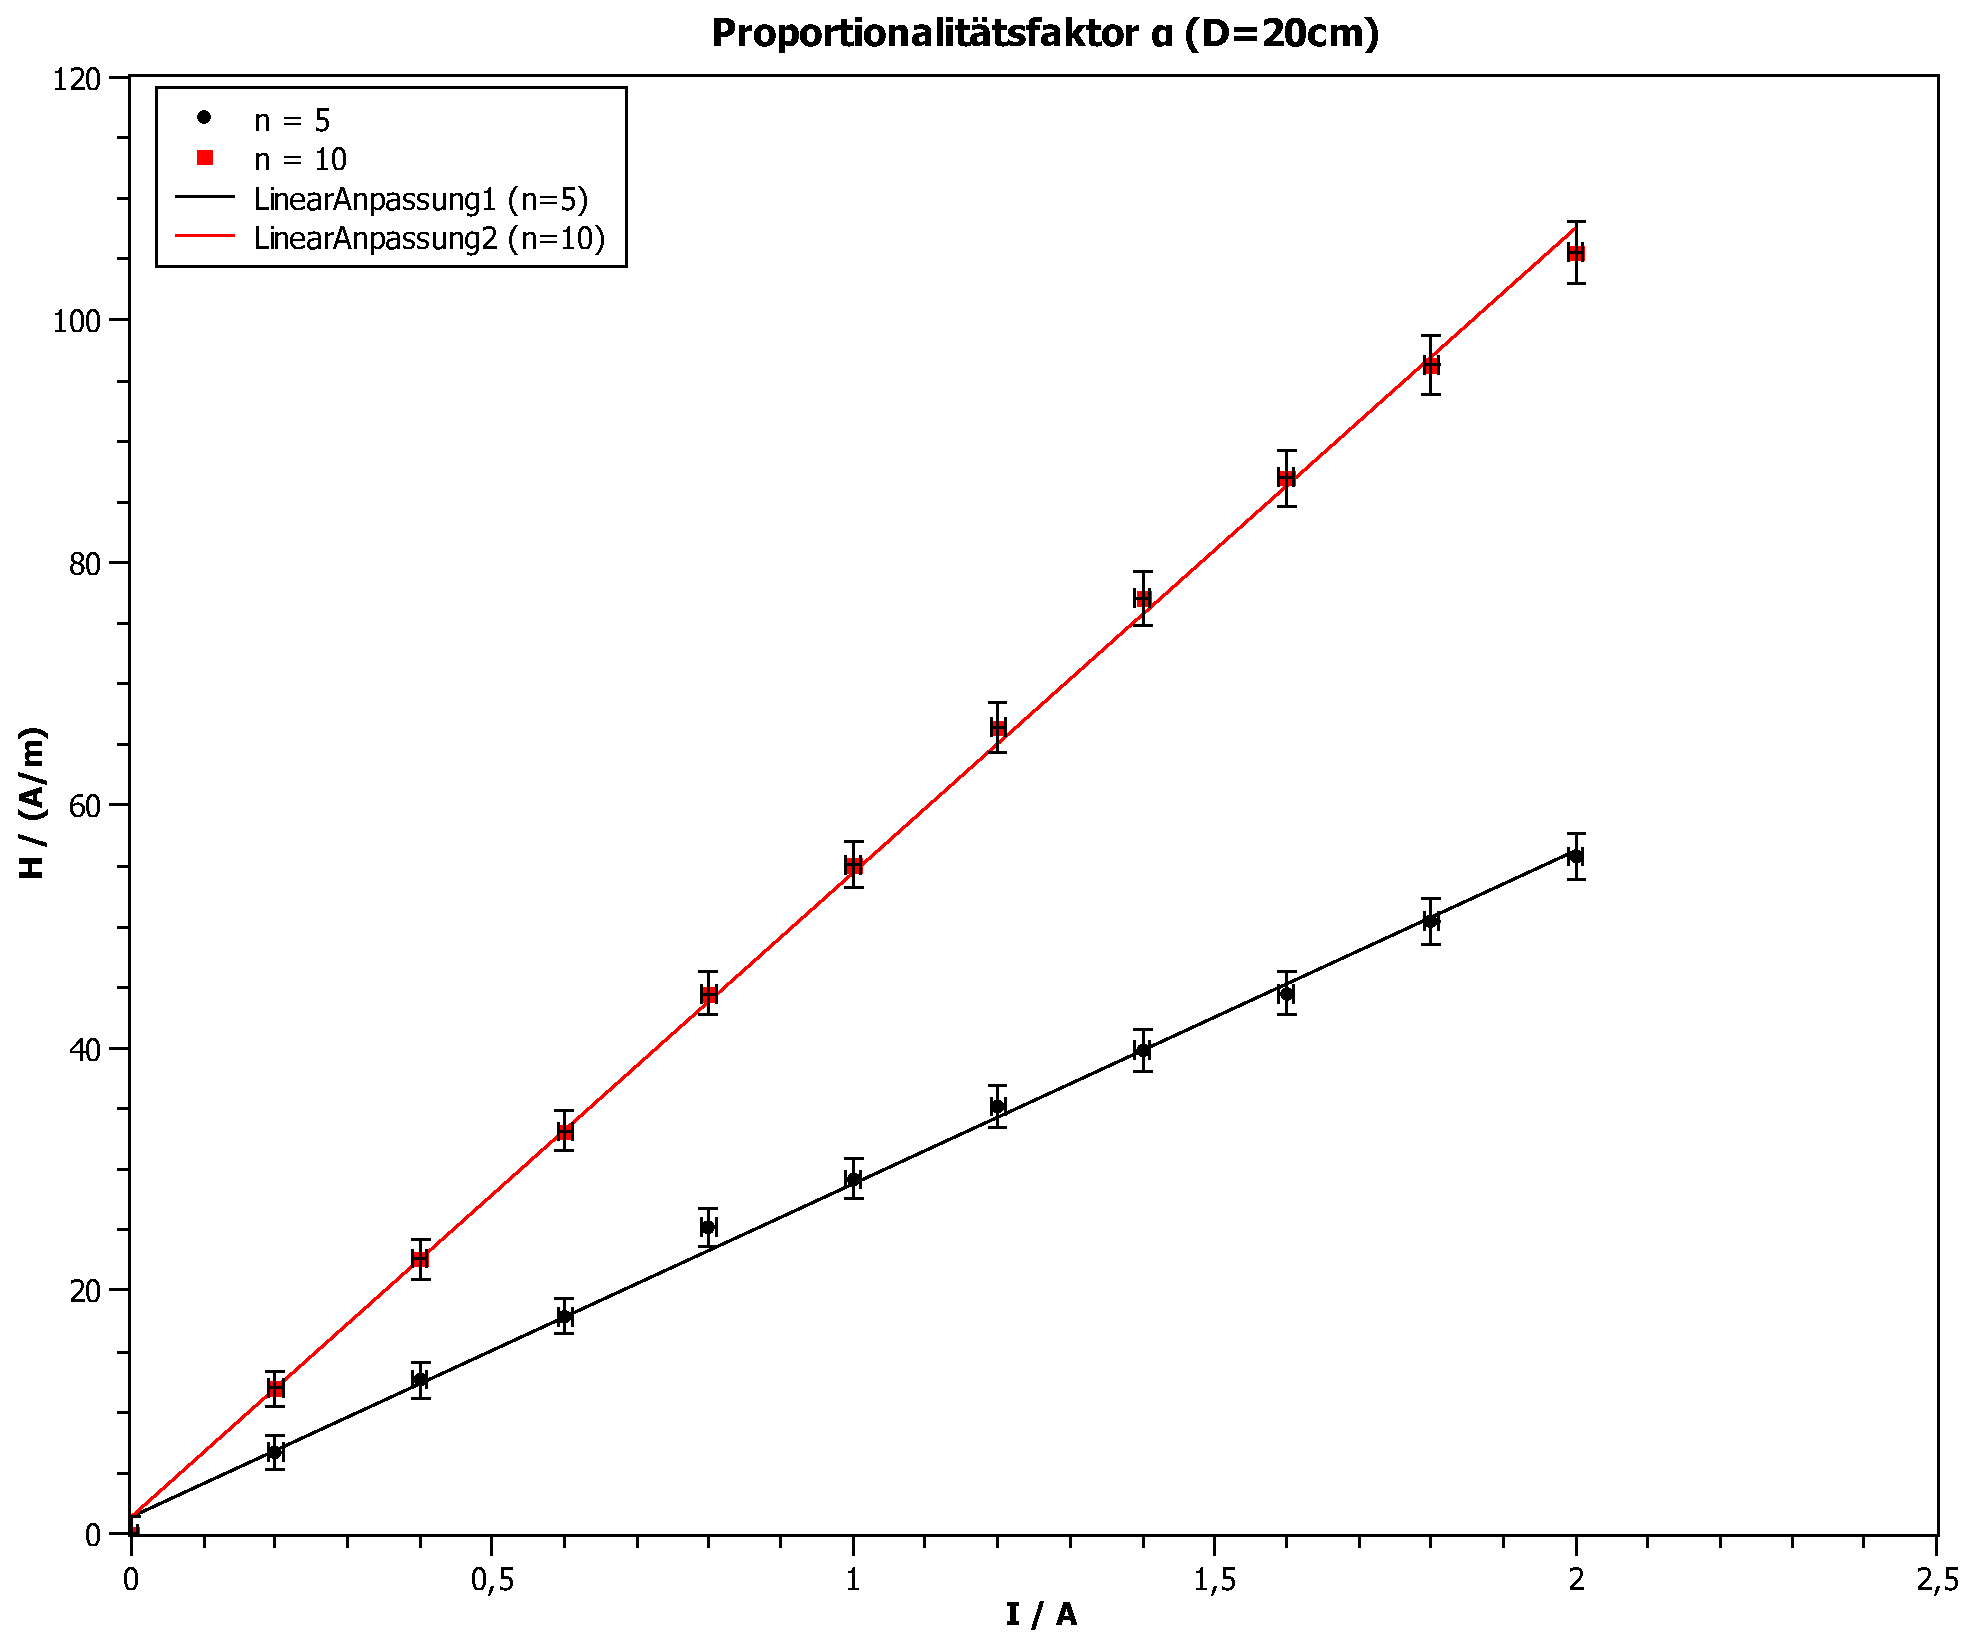
\includegraphics[width=.7\textwidth]{prop20.pdf}
    \caption[Proportionalitätsfaktor für D=20cm]{Proportionalitätsfaktor $\alpha$ für die kurze Spule mit $D=\SI{20}{cm}$.}
    \label{fig:20prop}
\end{figure}

\par\bigskip

\begin{figure}[H]
    \centering
    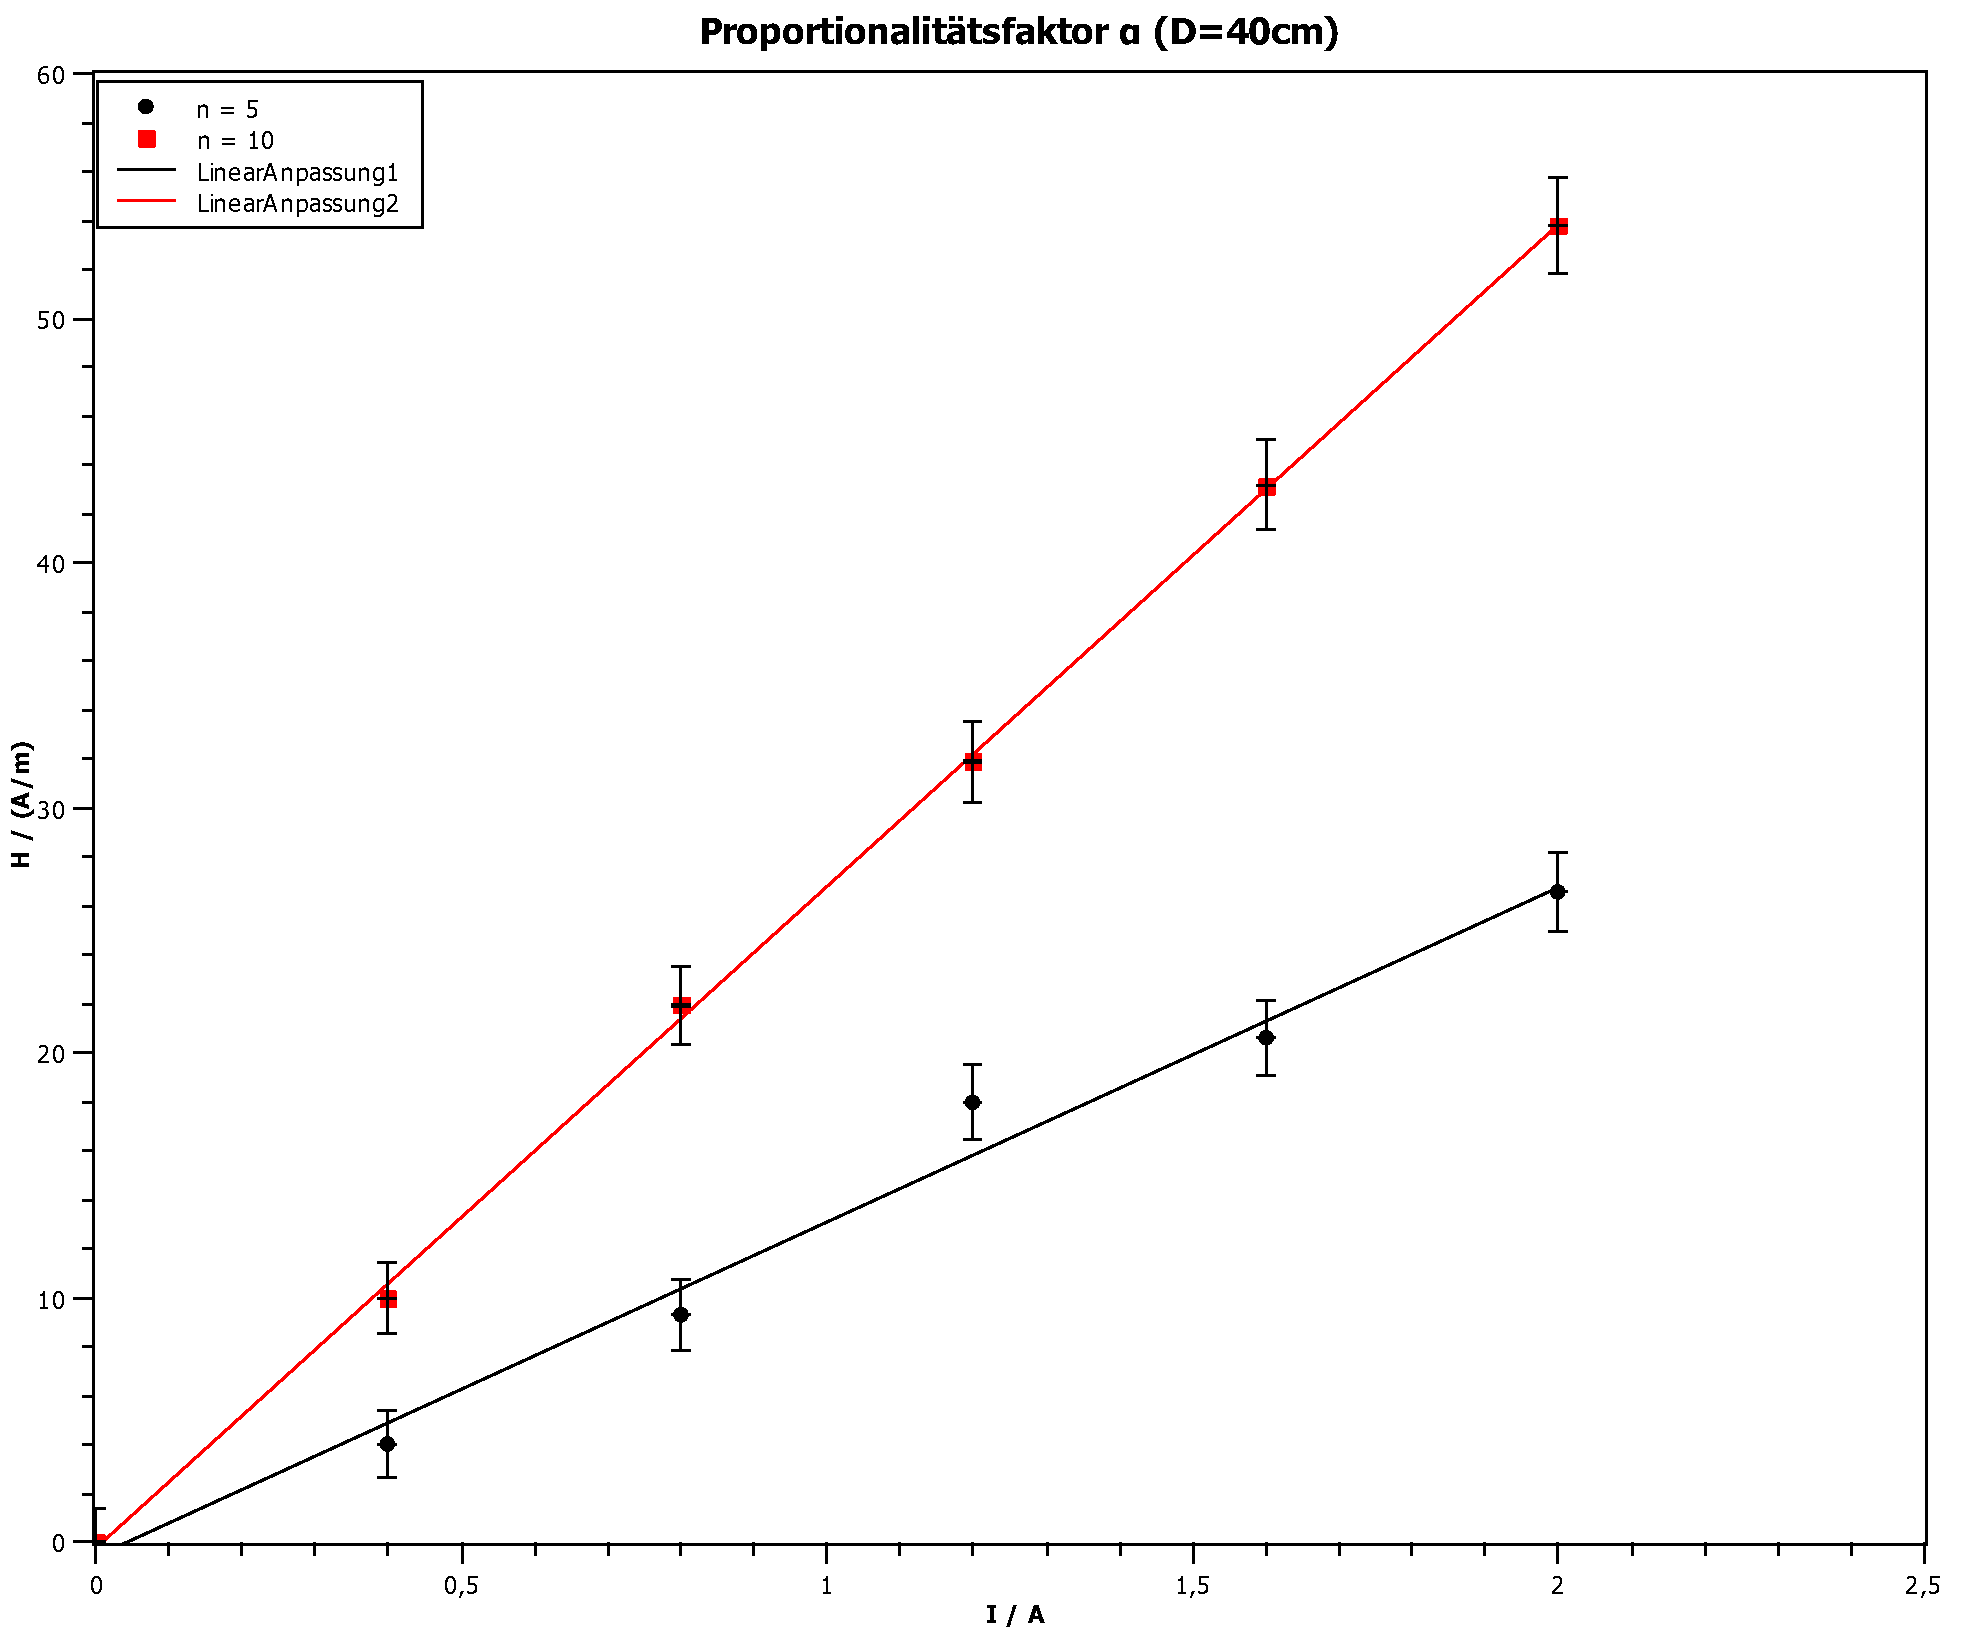
\includegraphics[width=.7\textwidth]{prop40.pdf}
    \caption[Proportionalitätsfaktor für D=40cm]{Proportionalitätsfaktor $\alpha$ für die kurze Spule mit $D=\SI{40}{cm}$.}
    \label{fig:40prop}
\end{figure}

Mit \gl{eq:k} und den gemessenen Ausschlägen für die kurzen Spulen lassen sich ihre magnetische Feldstärken $ H $ ermitteln
und als Funktion des Spulenstroms $ I $ in ein Diagramm (vgl. \bild{fig:20prop} und \bild{fig:40prop}) auftragen. Die
durch eine lineare Anpassunge resultierende Steigung $ m $ liefert mit \gl{eq:4} folgenden Zusammenhang:
\begin{equation}
    m = \frac{H_k}{I} = \alpha \cdot \frac{n}{R}
\end{equation}

und umgestellt nach $ \alpha $:
\begin{equation}
    \alpha = m \cdot \frac{R}{n} = m \cdot \frac{D}{2n}
\end{equation}
$\alpha$ ist hier als Faktor zu verstehen. In \gl{eq:test} wird beispielhaft der Spulenstrom aus \tabelle{tab:mess2} Zeilen Nr. 6
eingesetzt und das resultierende Feld mit dem zuvor ermittelten Kalibrierfaktor multipliziert.
\begin{equation}
    A = \frac{I \cdot N}{R} \cdot k
    = \frac{\SI{1,2}{A} \cdot 10}{\SI{0,1}{m}} \cdot \SI{0,151}{m^{-1}}
    = \SI{18,12}{Skt}
    \label{eq:test}
\end{equation}
Gemessen wurden hier jedoch \SI{10}{Skt}. Die Diskrepanz lässt sich durch die Inhomogenität des Feldes der kurzen Spule
in Kombination mit der Beschaffenheit des Versuchsaufbaus erklären. \gl{eq:4} in \gl{eq:8} eingesetzt zeigt
\begin{equation}
    \varphi = \frac{\phi_1 \cdot s}{d} \cdot \frac{I \cdot n}{R} \quad \Rightarrow \quad \alpha \, \widehat{=} \, \frac{\phi_1 \cdot s}{d}
\end{equation}
Der Wert $\alpha$ korrigiert also um die räumliche Ausdehnung des Stabmagneten, seine eigene Polstärke und den Einfluss
des Direktionsmomentes des Torsionsdrahts.
\par\medskip
Für die vier Messungen an den kurzen Spulen ergeben sich folgende Werte für den Proportionalitätsfaktor $\alpha$:
\vspace{5mm}
\begin{table}[h]
    \centering
    \caption[Proportionalitätsfaktoren]{Steigungen der Ausgleichsgeraden und korrespondierende Werte für den Proportionalitätsfaktor $\alpha$}
    \begin{tabular}{@{}llll@{}}
        \toprule
        \multicolumn{2}{l}{}                       & $(m \pm \Delta m) / m^{-1}$  & $\alpha$ \\ \midrule
        \multirow{2}{*}{$D=\SI{20}{cm}$} & $n=5$   & $27,4 \pm 0,4$               & 0,548    \\
                                         & $n=10$  & $53,1 \pm 0,5$               & 0,531    \\
        \multirow{2}{*}{$D=\SI{40}{cm}$} & $n=5$   & $13,7 \pm 0,8$               & 0,548    \\
                                         & $n=10$  & $27,0 \pm 0,3$               & 0,540    \\ \cmidrule(l){1-4} 
    \end{tabular}
\end{table}

\section{Messunsicherheiten}
Die durch die Messeinrichtung gegebenen Messfehler sind
\begin{align*}
    \Delta L &= \pm \SI{0,001}{m} &\quad& \text{Fehler bei der Längenmessung (Stahllineal).}\\
    \Delta A &= \pm \SI{0,2}{Skt} &\quad& \text{Fehler bei der Auslenkung durch Skalenteilung und Leuchtpunkt.}\\
    \Delta I &= \pm \SI{0,01}{A}  &\quad& \text{Fehler des Spulenstroms durch Ungenauigkeit der Stromquelle.}
\end{align*}

Der größte Fehler für die magnetische Feldstärke $ H $ ergibt sich bei der langen Spule mit der Windungszahl $ n=240 $ gegeben
durch die Messunsicherheiten aus Spulenstrom $I$ und Spulenlänge $L$ zu:
\begin{align}
    \Delta H    &= \left\vert\frac{\delta H}{\delta I}\right\vert \cdot \Delta I + \left\vert\frac{\delta H}{\delta L}\right\vert \cdot \Delta L \nonumber\\
                &= \frac{n}{L} \cdot \Delta I + \frac{n \cdot I}{L^{2}} \cdot \Delta L \nonumber\\
                &= \frac{240}{\SI{0,615}{m}} \cdot \SI{0,01}{A} + \frac{240 \cdot \SI{0,7}{A}}{(\SI{0,615}{m})^2} \cdot \SI{0,001}{m}\nonumber\\
                &= \SI{4,34}{\frac{A}{m}} \nonumber
\end{align}



Der größte Fehler für den Proportionalitätsfaktor $\alpha$ zeigt sich bei der kurzen Spule mit 40 cm Durchmesser und 5 Windungen:
\begin{align}
    \Delta \alpha   &= \left\vert\frac{\delta \alpha}{\delta m}\right\vert \cdot \Delta m \nonumber\\
                    &= \frac{D}{2 \cdot n} \cdot \Delta m \nonumber\\
                    &= \frac{\SI{0,4}{m}}{2 \cdot 5} \cdot \SI{0,8}{m^{-1}} \nonumber\\
                    &= 0,032 \nonumber
\end{align}
\chapter{Fazit}
Der Versuch konnte ein tieferes Verständniss über die Zusammenhänge zwischen Spulengeometrien und den resultierenden
Feldstärken vermitteln. Interessant war auch, zu sehen wie schnell sich eine scheinbar geringe Änderung des Spulenstromes
auf die Feldstärke auswirkt.
\par
\hspace{1cm}Zu vermissen war eine - wenn auch für den konkreten Versuch nicht notwendige - Möglichkeit zur Kalibrierung
des Rückstellmomentes der Torsionsfeder. Weiter ist ein einstellbarer Diodenstrom des Lasers oder ein dunklerer Grund der
Skala wünschenswert. Da der Laser im Istzustand einen relativ großen und hellen Leuchtpunkt erzeugt, erhöht er so unnötig
den Messfehler der Auslenkung und trägt darüber hinaus auch zur Ermüdung der Augen des Experimentators bei.
%-------------------
\newpage
\listoffigures 
\listoftables
\addchap{Verwendete Symbole}

\begin{table}[h]
    \begin{tabular}{@{}ll@{}}
        \(A\)           & Auslenkung                                                                          \\
        \(D\)           & Spulendurchmesser                                                                   \\
        \(F_{mag}\)   & Magnetkraft                                                                         \\
        \(H\)           & Magnetische Feldstärke                                                              \\
        \(H_k\)         & Magnetische Feldstärke der kurzen Spule                                             \\
        \(H_l\)         & Magnetische Feldstärke der langen Spule                                             \\
        \(I\)           & Spulenstrom                                                                         \\
        \(L\)           & Länge der Spule                                                                     \\
        \(M_{mag}\)   & Durch Magnetkraft verursachtes Drehmoment                                           \\
        \(M_{Rück}\)  & Rückstellmoment                                                                     \\
        \(R\)           & Radius der Spule                                                                    \\
        \(d\)           & Direktionsmoment                                                                    \\
        \(k\)           & Kalibrierfaktor                                                                     \\
        \(m\)           & Steigung der AUsgleichsgeraden                                                      \\
        \(n\)           & Windungszahl                                                                        \\
        \(r\)           & Hebelarmlänge                                                                       \\
        \(s\)           & Länge des Stabmagneten                                                              \\
        \(x\)           & Position entlang der Spulenachse \\
        & \\
        \(\Delta A\)  & Fehler der Ausschlagsmessung \\
        \(\Delta H\)  & Fehler der Feldstärke \\
        \(\Delta I\)  & Fehler des Spulenstrom \\
        \(\Delta L\)  & Fehler der Längenmessung \\
        \(\Delta k\) & Fehler des Kalibrierfaktors \\
        \(\Delta \alpha\) & Fehler des Proportionalitätsfaktors \\
        \(\alpha\)    & Proportionalitätsfaktor                                                               \\
        \(\beta\)     & Winkel zwischen Spulenachse und Ortsvektor des Spulenradius in negativer x-Richtung   \\
        \(\gamma\)    & Winkel zwischen Spulenachse und Ortsvektor des Spulenradius in positiver x-Richtung   \\
        \(\phi\)      & Magnetischer Fluss                                                                  \\
        \(\varphi\)   & Auslenkungswinkel                                                                   \\
        \(\mu_0\)     & Absolute Permeabilität                                                              \\
    \end{tabular}
\end{table}
\appendix
\chapter{Anhang}
%
\begin{table}[ht]
    \centering
    \caption[Messung lange Spule]{Messwerte Teil 1: Lange Spule (\(L=\SI{0,615}{m}\))}
    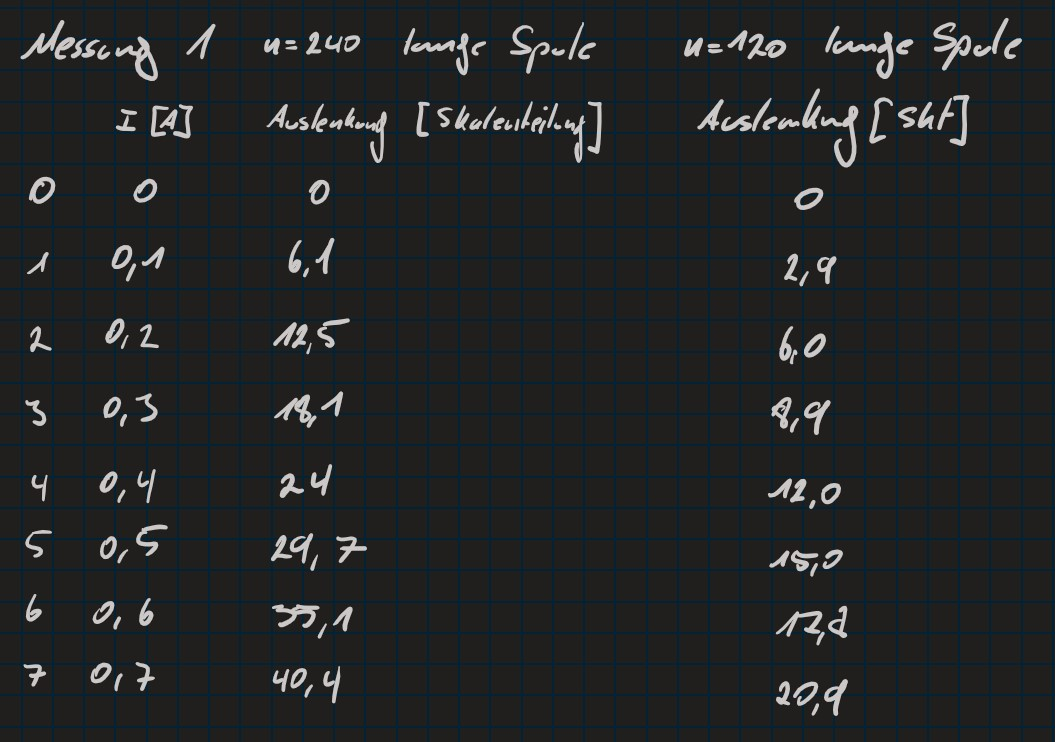
\includegraphics[width=.8\textwidth]{messungen/messung1.jpg}
    \label{tab:mess1}
\end{table}
%
\begin{table}[ht]
    \centering
    \caption[Messung kurze Spule \(D=\SI{0,2}{m}\)]{Messwerte Teil 2: Kurze Spule (\(D=\SI{0,2}{m}\))}
    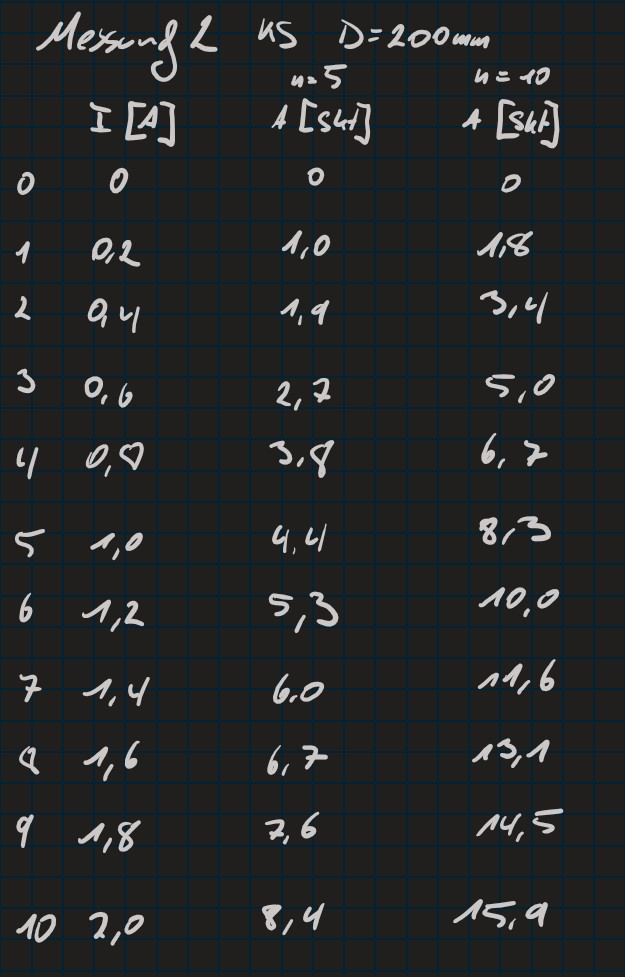
\includegraphics[height=.75\textheight]{messungen/messung2.jpg}
    \label{tab:mess2}
\end{table}
%
\begin{table}[ht]
    \centering
    \caption[Messung kurze Spule \(D=\SI{0,4}{m}\)]{Messwerte Teil 3: Kurze Spule (\(D=\SI{0,4}{m}\))}
    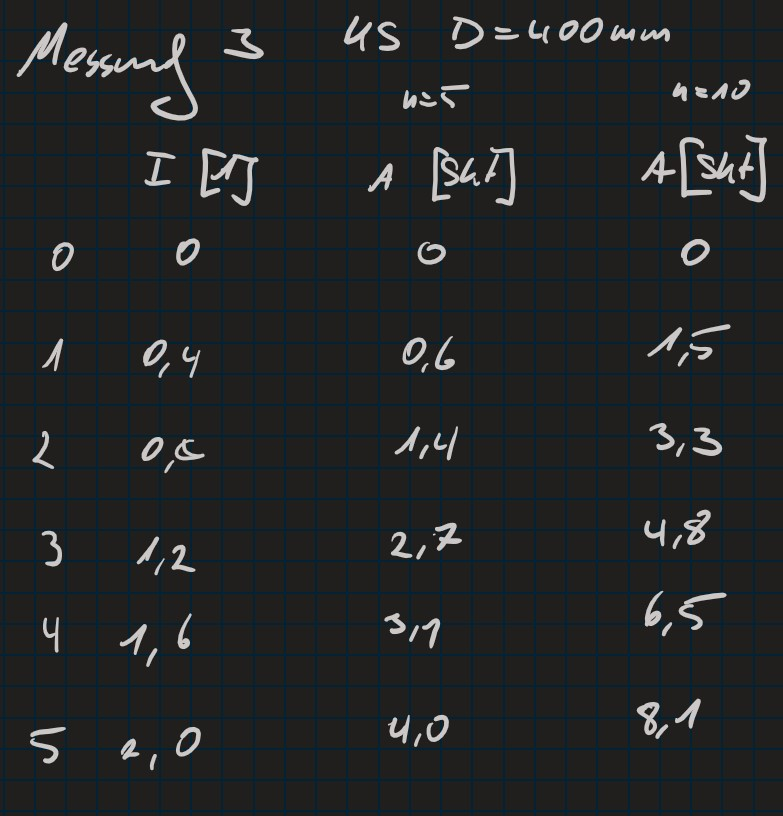
\includegraphics[height=.5\textheight]{messungen/messung3.jpg}
    \label{tab:mess3}
\end{table}%
\printbibliography%
%\bibliographystyle{plaindin}
%==========================================
\end{document}